\chapter{Experiment}
%todo make sure you explain the optimization
% -    Whenever you describe these, you need to list, and precisely describe: the contender models, and how they were trained/tuned; the performance metrics; the evaluation setup, including data and re-sampling for performance estimation
% -    There’s probably something wrong with he LRN layer, please check.
% -    If you use dropout, you may have to adjust learning rates, please check. Not doing so would explain bad results.

% A few experiments where held to compare performance such as Local response normalization vs batch normalization.

\section{LRN vs Batch normalization}
For all models described in \citep{KarpathyCVPR14} which includes the single frame, early fusion, late fusion and slow fusion models. A version was constructed with the proposed local response normalization.  An equivalent model for each model was also constructed where the  local response normalization layers were replaced by the more relevant batch normalization layer.
Both model types used sparse categorical cross entropy loss and the same parameters for stochastic gradient descent which includes a   momentum of 0.9,  decay of 0.0005 and a learning rate of $1e^{-3}$.  
The train data was split into a batch size of about 32 and the elements were randomly shuffled.
All models were set to run for 20 epochs, and early stopping was implemented for all models to stop at an accuracy of 99\%. All models were ran on the UCL cluster with the scripts using Batch scripts that required 128GB, and 2 GPUs. The single frame and early fusion jobs were set to run for about 12 hours while the late and slow fusion jobs were also set to run for 20 hours on the clusters.
In this experiment, the performances of the model were only evaluated against their performance on the training data.

\section{Temporal relationships}
%todo make sure you explain the optimization
Here, the performance of the single frame, late fusion, early fusion and slow fusion models using the batch normalization layers,  were validated against the test data. These were the models trained in the previous experiment.  This experiment was done to compare the performances of these models as they vary in how they take into account temporal features as done in \citep{KarpathyCVPR14}.

\section{Optimization methods}
%todo link to theory section on optimization and talk about the way you decided on the values
This experiment involved testing out the performance of different optimization methods using the single frame model with batch normalization.
 Models using the below optimization techniques were built, and their performance was compared to the previous single frame model with batch normalization and stochastic gradient descent.
\begin{itemize}
%maybe add the AMSGrad variant%
    \item Model with Adam optimization -  At first the default parameters such as the learning rate of 0.001, $\beta_1$ of 0.9, $\beta_2$ of 0.999  $\epsilon$ of $10^-8$ and decay of 0 were used. However, after some experimentation with a few learning rates a factor of 10 away, a final learning rate of 1 was used. 
    \item Model with RMS prop - this used the default parameters such as the learning rate of 0.001, $\rho$ of 0.9, $\epsilon$ of $10^-8$ and a  decay=0
\end{itemize}
These models were trained for about 10  epochs using an early stopping for a stop at an accuracy of 99\%. All models also ran on the UCL cluster using 128GB of RAM and 2 GPUs. 


\section{Random single frame}
%todo calculation for the video length for the random generator min clips is 1.06, 25fp so 26%
\cite{KarpathyCVPR14},  talks about how the single frame model was better than most models, suggesting that local motion cues from the temporal features may not be critically important. Hence implying that models that take into account temporal features might not be necessary and as a further study, this is something to be investigated.
This experiment tries to look into this by randomly selecting a random image from one video and passing this an input into the single frame model. 
Becuase length of videos in the UCF101 dataset varies extensively. This random image was selected from the first 25 frames. This was because the minimum the shortest video was 1.06 seconds and the frames were taken at 25 frames per second as discussed in \citep{soomro2012ucf101}.
The model ran using stochastic gradient descent with a momentum of 0.9,  decay of 0.0005 and a learning rate of $1e^{-3}$.  
The train data was split into a batch size of about 32 and the elements were randomly shuffled.
The model was set to run for 10 and 20 epochs, and early stopping was implemented for the model to stop at an accuracy of 90\%.
It also ran on the UCL cluster using 128GB of RAM and 2 GPUs. 


\section{Performance of pre-trained models}
% todo how the learning rate was decided
This experiment involved comparing the performances of the previously discussed pre-trained models, which include VGG19, mobileNetv2, inception, ResNet. The models were all trained with stochastic gradient descent and a sparse categorical cross-entropy loss for about five epochs. Early stopping was used, where models we set to stop at a 90\% accuracy. A dropout of 50\% was used by all models. The models were also trained with stochastic gradient descent with a learning rate of 0.1. The learning rate was decided after experimenting with learning rates of a faction of 10, starting with the learning rate of $1e^-3$. A momentum of 0.9 and decay of 0.0005 was also used. The architectural setup of these pre-trained model experiment can be seen in \ref{fig:pretrained-single}. This shows a frame being feed to the pre-trained model layer, which has a 50\% dropout applied to it, followed by a global average pooling layer and then the output layer. It also ran on the UCL cluster using 128GB of RAM and 2 GPUs. The training data was also put into batches of 32 and shuffled.  

\begin{figure}
    \centering
    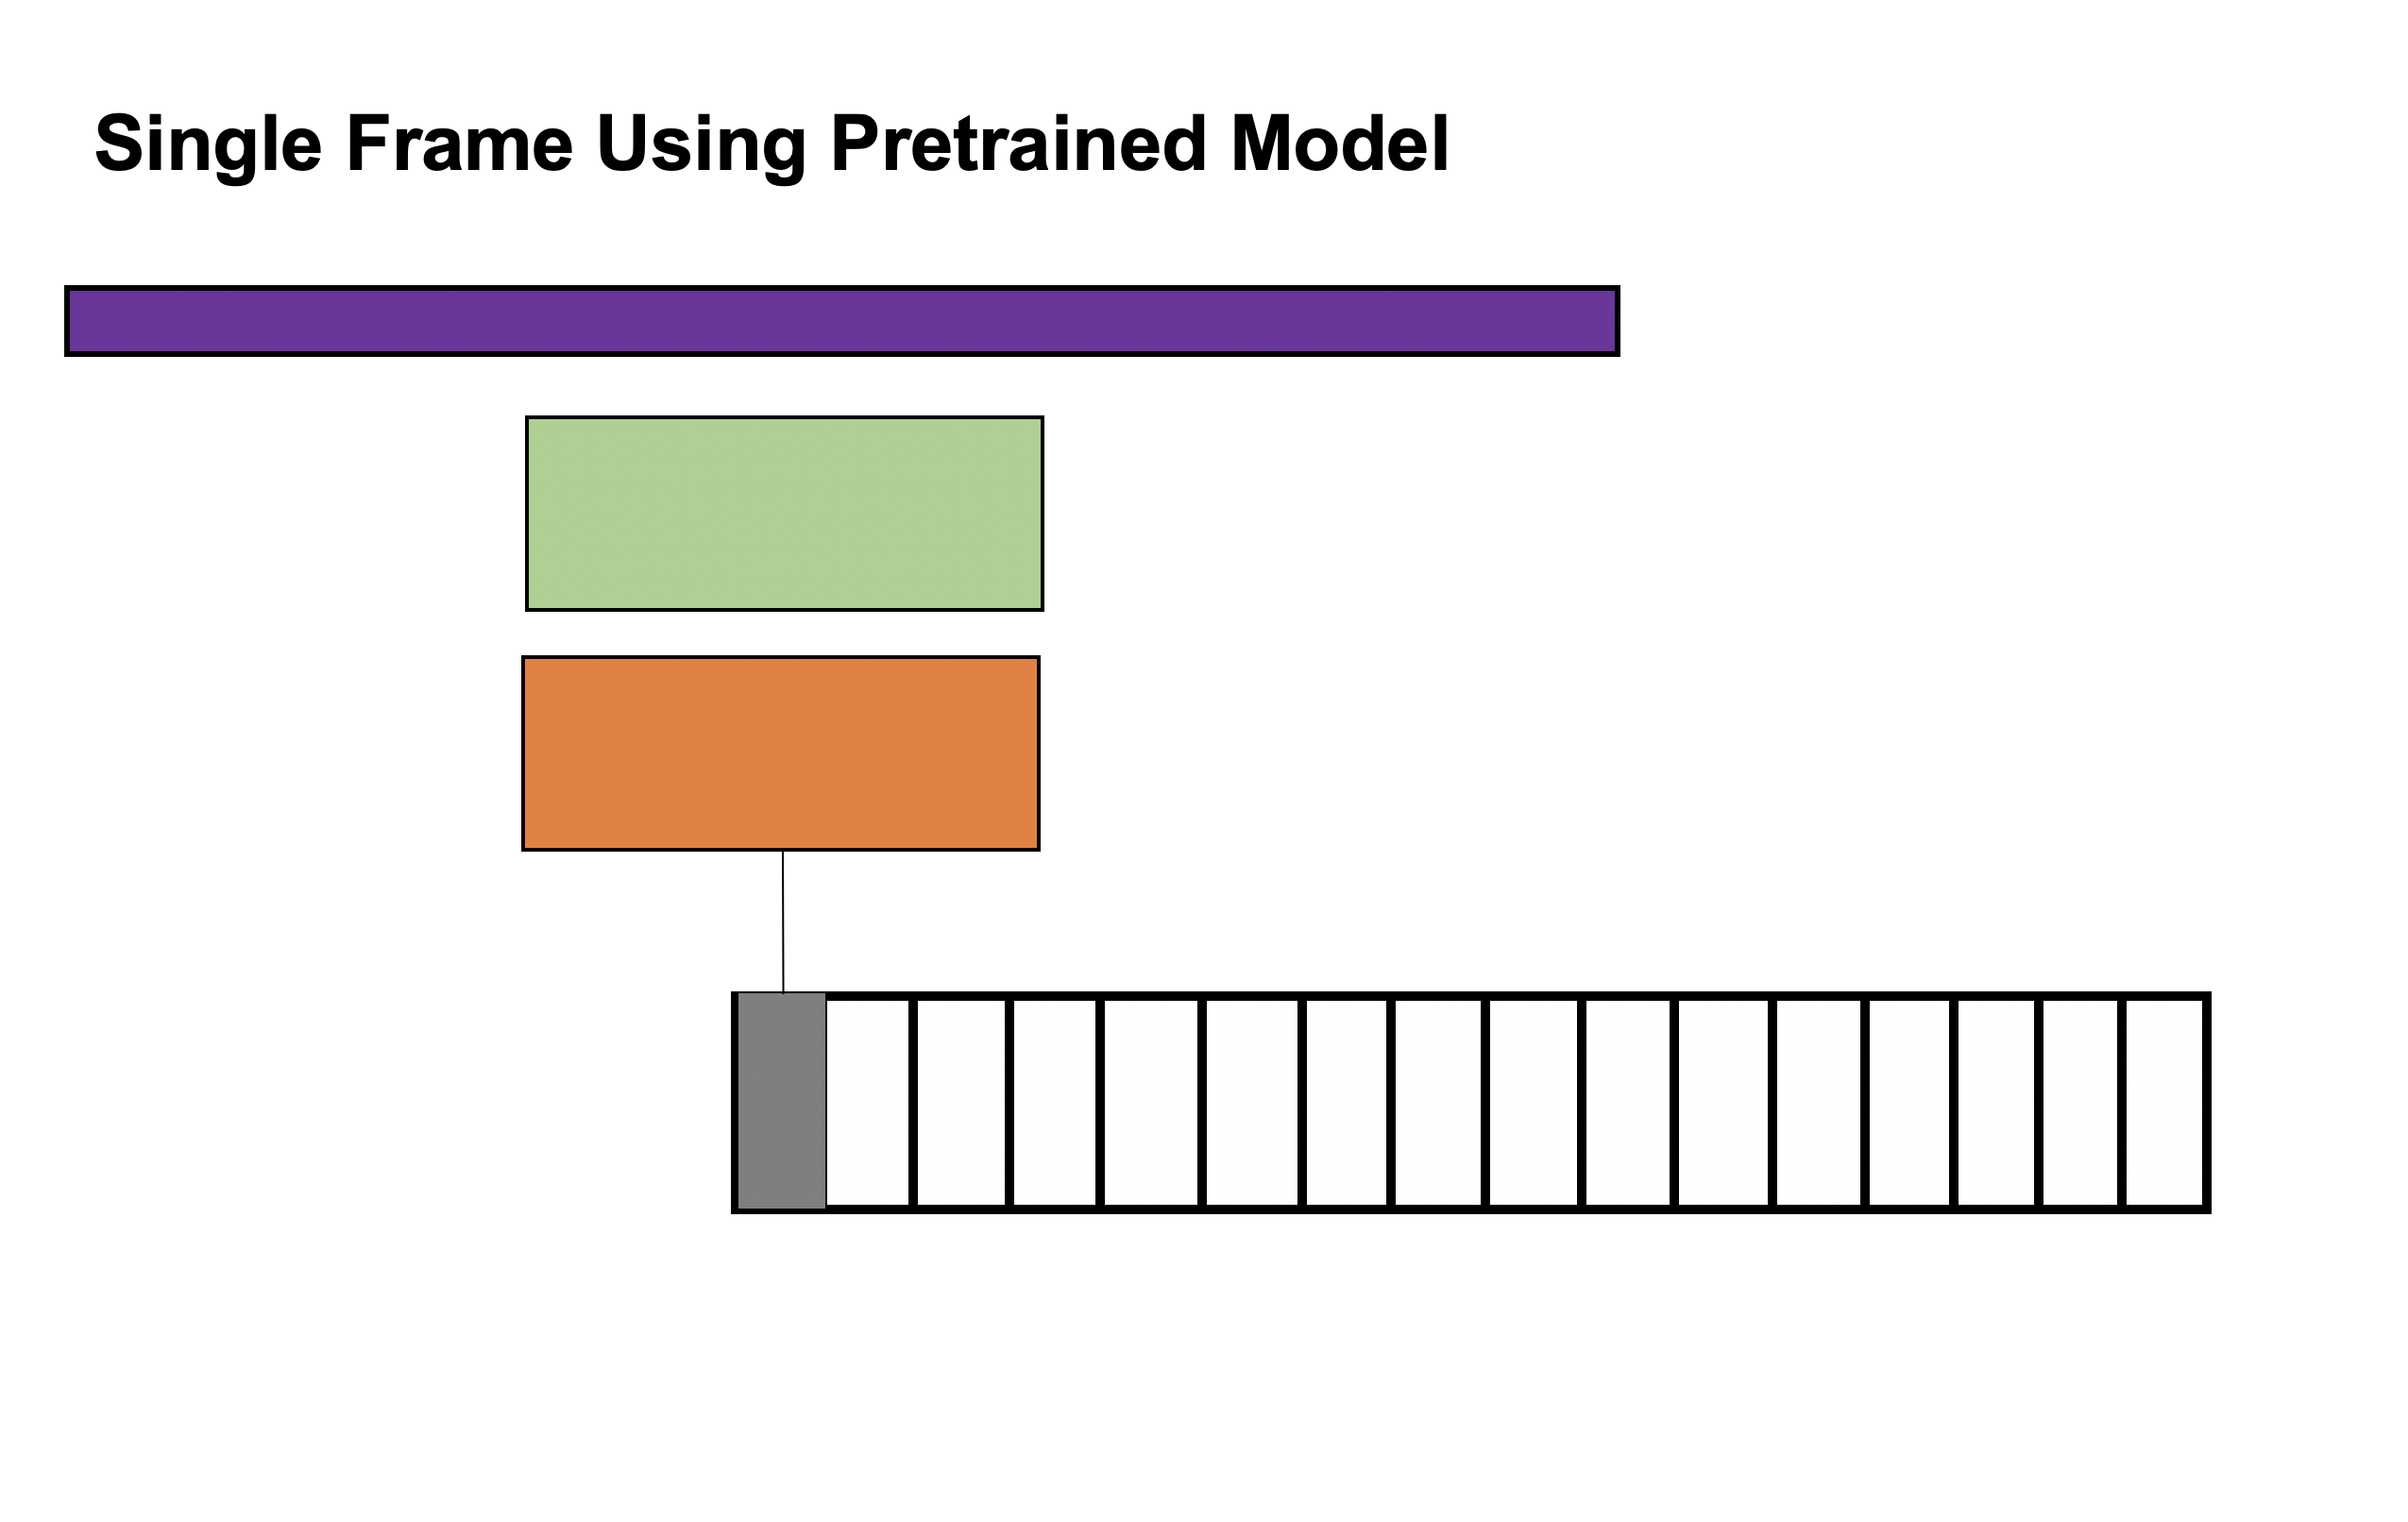
\includegraphics[width=75mm,scale=0.5]{pretrained-single.png}
    \caption{Architectural setup of the pre-trained models, the frame is feed to the pre-trained model layer which has a  50\% dropout applied to it, followed by a global average pooling layer and then the output layer. 
}
    \label{fig:pretrained-single}
\end{figure}


\section{Performance of pre-trained models with multi frames}
This experiment looks to add some temporal information to using the pre-trained models discussed previously.  This setup was inspired by the late fusion model in \citep{KarpathyCVPR14} and involved selecting two frames 15 frames apart. Each frame was then passed through a layer with the same pre-trained model using a dropout of 50\%.  This was then combined and passed to the global average pooling layer as seen in figure \ref{fig:pretrained-late}. This experiment was done for the VGG19, mobileNetv2, inception, ResNet. 
The models were trained similar to the previous experiment using stochastic gradient descent with a learning rate of 0.1, momentum of 0.9,  decay of 0.0005 . These models also ran on the UCL cluster using 128GB of RAM and 2 GPUs.

\begin{figure}
\centering
    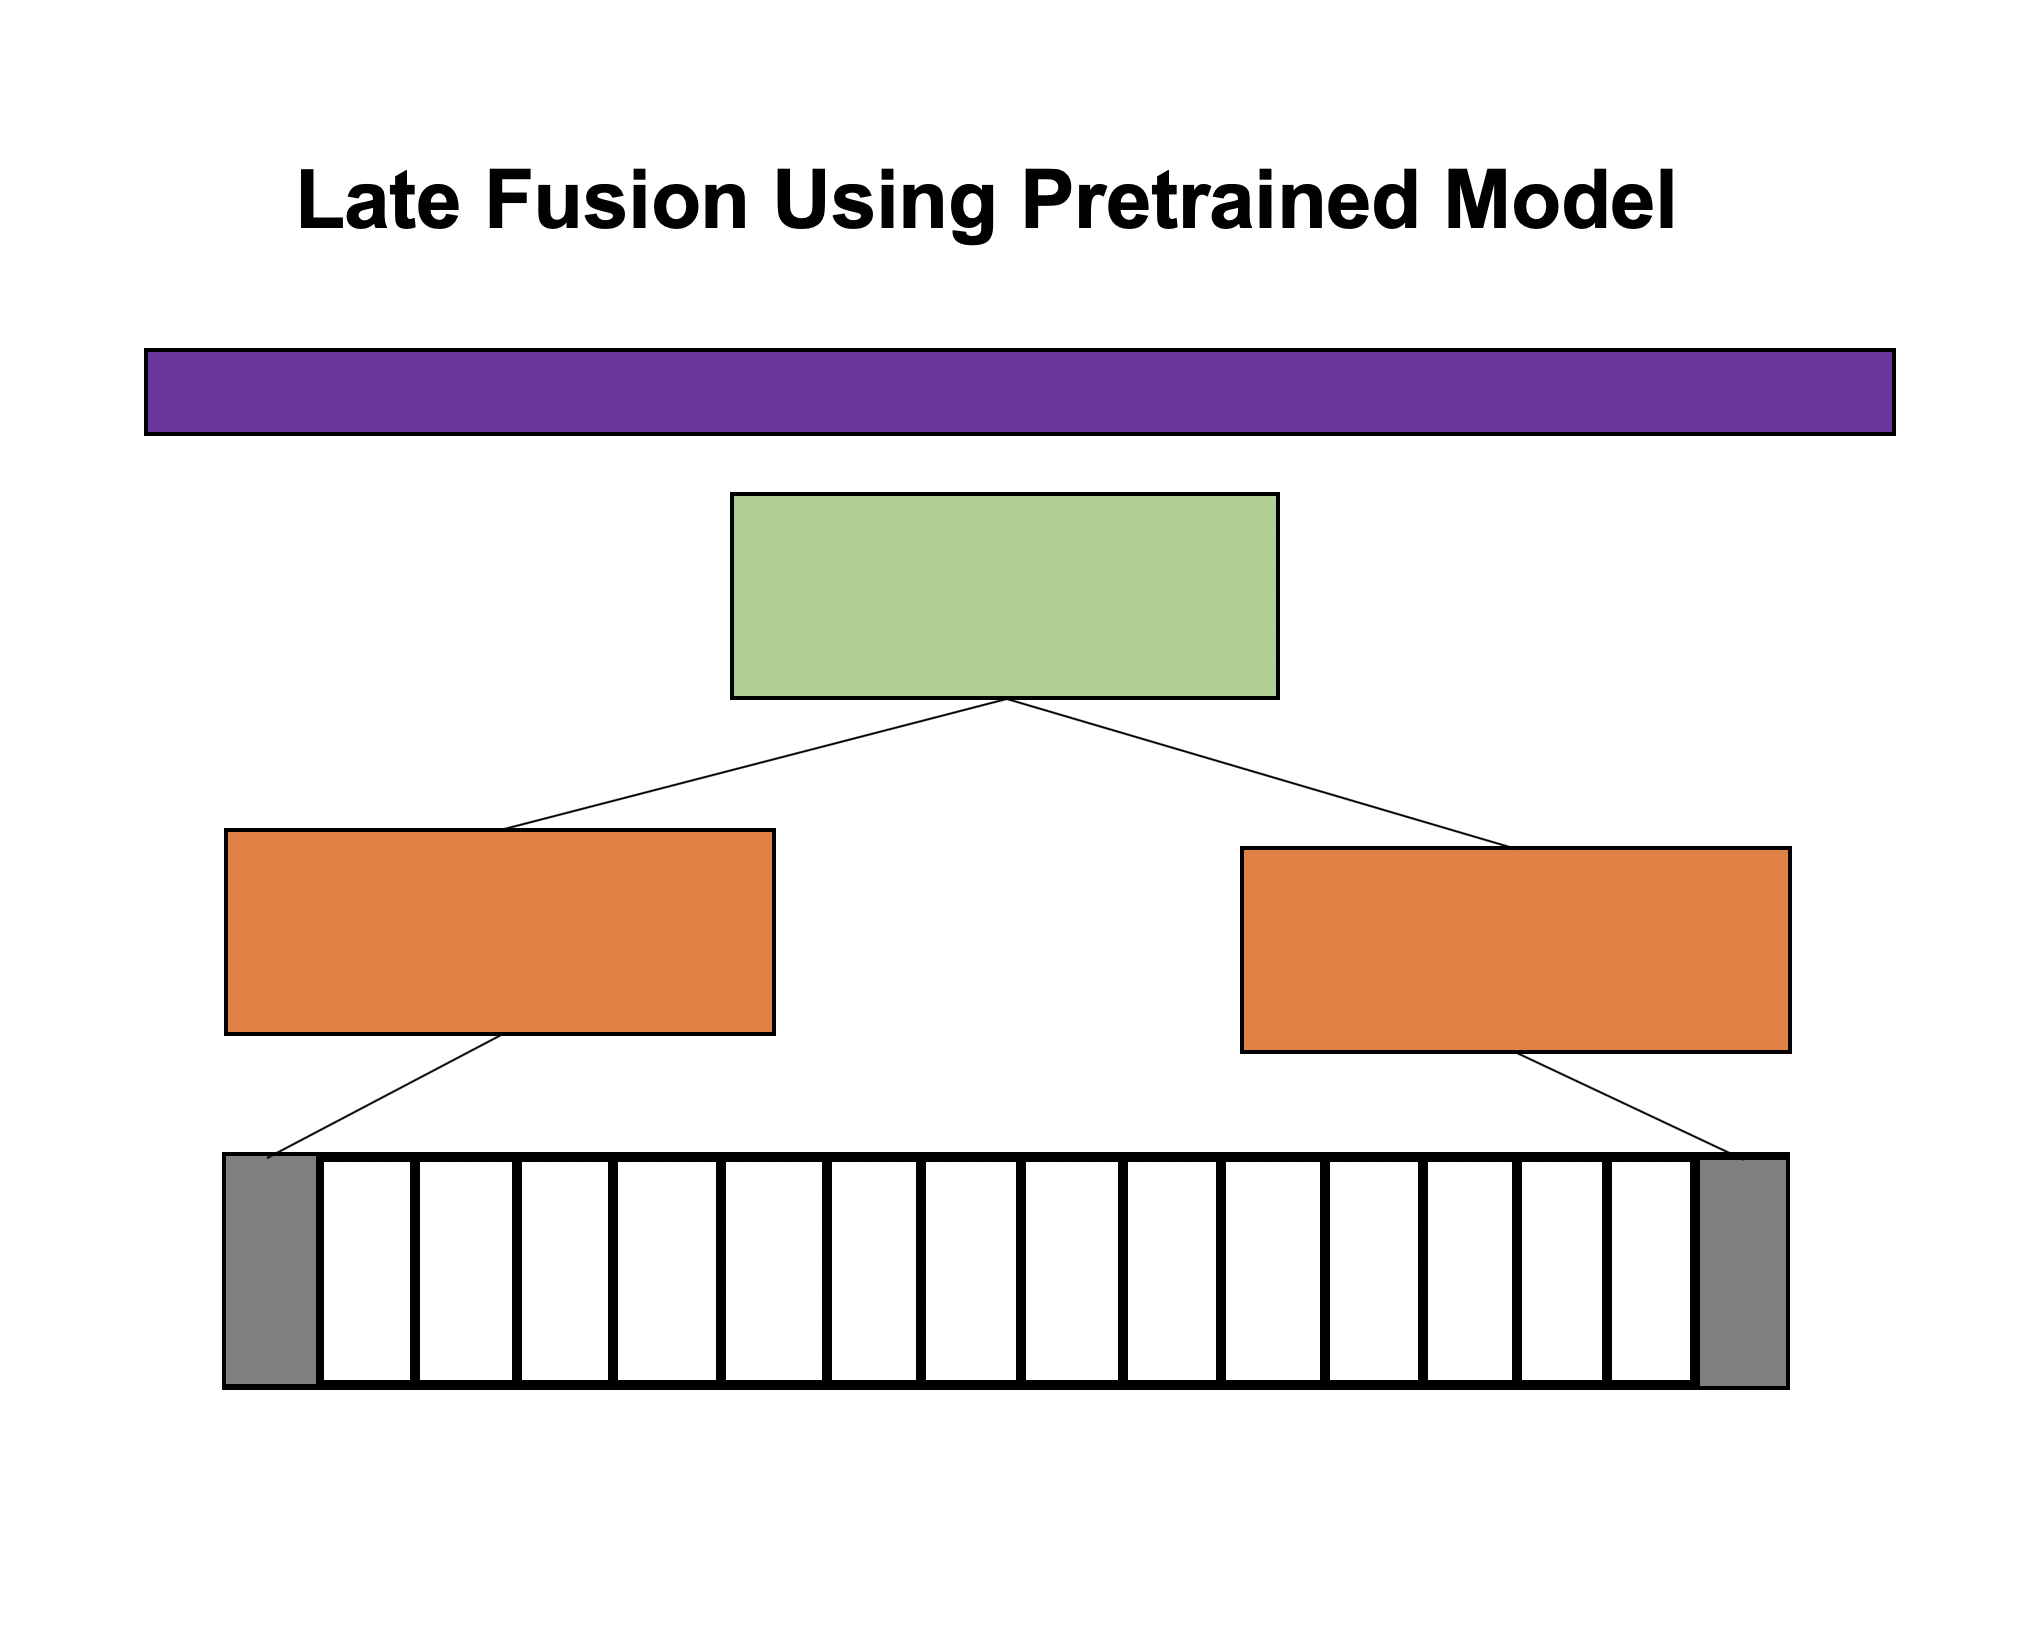
\includegraphics[width=75mm,scale=0.5]{pretrained-late.png}
    \caption{Structure of pre trained late fusion models}
    \label{fig:pretrained-late}
\end{figure}


\section{Data Augmentation}
%t need to find papers for the 255 thing%
\citep{KarpathyCVPR14} paper talks about using certain augmentation on data. The augmentation, as discussed in the setup chapter of this report, were attempted using tensorflow libraries image library on the training dataset. The preprocessed were then applied to the training data for a single frame model using batch normalization and stochastic gradient descent with a momentum of 0.9,  decay of 0.0005 and a learning rate of $1e^{-3}$.  This model was then validated again the test set. And was ran on the UCL cluster using 128GB of RAM and 2 GPUs.




%\section{Data Augmentation}
%To improve traing time different cluster configures where used with different ram sized cpu vs gpu and parallel machines%



% \subsection{RNN}
% trying
